\begin{pastexam}[label={px:ncku-112-isec-ds-02}]{成大智慧資安學程 112 學年度 第 2 題}
（問答）

(10\%) Write the prefix and postfix form of the following expressions:\\
(a) (A*B)/D+E*(f*A+D)-C\\
(b) \texttt{!((a \&\& c) || (c > d))} \qquad\qquad // assuming C precedence
\end{pastexam}

\begin{pastsoln}
答案：
\begin{center}
\begin{tabular}{lll}
\toprule
 & 前序（prefix） & 後序（postfix） \\
\midrule
(a) & \texttt{- + / * A B D * E + * f A D C} & \texttt{A B * D / E f A * D + * + C -} \\
(b) & \texttt{! || \&\& a c > c d} & \texttt{a c \&\& c d > || !} \\
\bottomrule
\end{tabular}
\end{center}
做法用資結書第~6.3~節的「加滿括號」：先依優先順序和結合性替每個運算加一對括號，再把運算子
搬到它那對括號的左括號（前序）或右括號（後序），最後擦掉括號。 運算式樹（資結書第~7.7~節）的
前序、後序走訪給出同樣的結果，下面兩種都寫。

\textbf{(a)} \texttt{*}、\texttt{/} 的優先順序高於 \texttt{+}、\texttt{-}，同級的由左往右結合。
\begin{enumerate}
\item 原式的括號先保留：$(A*B)$ 和 $(f*A+D)$；後者裡面 \texttt{*} 先算：$((f*A)+D)$。
\item 第一層的 \texttt{/} 和 \texttt{*}：$((A*B)/D)$、$(E*((f*A)+D))$。
\item 剩下的 \texttt{+}、\texttt{-} 同級，由左往右：先 \texttt{+} 後 \texttt{-}。
\end{enumerate}
加滿括號後是
\[
\Bigl(\bigl(((A*B)/D) + (E*((f*A)+D))\bigr) - C\Bigr).
\]
對應的運算式樹：
\begin{center}
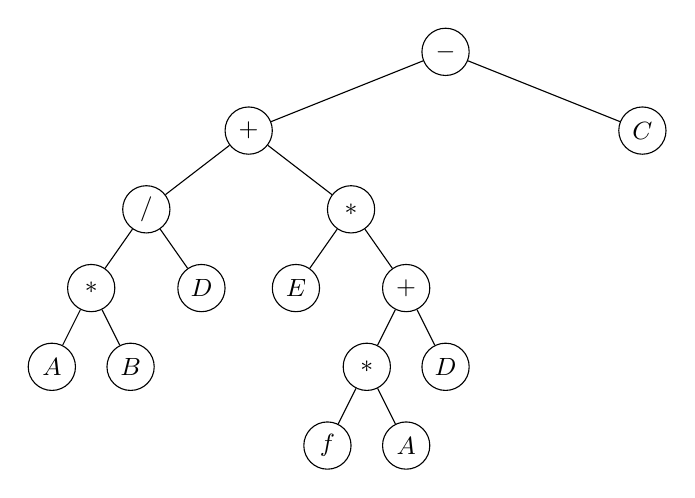
\begin{tikzpicture}[level distance=10mm,
  every node/.style={circle,draw,inner sep=0pt,minimum size=6mm,font=\small},
  level 1/.style={sibling distance=50mm},
  level 2/.style={sibling distance=26mm},
  level 3/.style={sibling distance=14mm},
  level 4/.style={sibling distance=10mm}]
\node {$-$}
  child {node {$+$}
    child {node {$/$}
      child {node {$*$} child {node {$A$}} child {node {$B$}}}
      child {node {$D$}}}
    child {node {$*$}
      child {node {$E$}}
      child {node {$+$}
        child {node {$*$} child {node {$f$}} child {node {$A$}}}
        child {node {$D$}}}}}
  child {node {$C$}};
\end{tikzpicture}
\end{center}
前序（根、左、右）：根 \texttt{-}，接左子樹 \texttt{+} 的前序 \texttt{+ / * A B D * E + * f A D}，
最後 \texttt{C}，得 \texttt{- + / * A B D * E + * f A D C}。 後序（左、右、根）：
左子樹 \texttt{A B * D / E f A * D + * +}，接 \texttt{C}，最後根 \texttt{-}，得
\texttt{A B * D / E f A * D + * + C -}。 三種寫法裡運算元的順序都是
$A, B, D, E, f, A, D, C$，和原式一致，可以用來檢查。

\textbf{(b)} C 的優先順序由高到低：一元的 \texttt{!}，關係運算 \texttt{>}，\texttt{\&\&}，
\texttt{||}。 本題每一層都已經有括號，優先順序只用來確認 \texttt{!} 是一元運算子、作用在後面整個
括號上。 加滿括號：
\[
\bigl(!\,\bigl((a \mathbin{\&\&} c) \mathbin{||} (c > d)\bigr)\bigr).
\]
運算式樹的根是 \texttt{!}，只有一個子節點 \texttt{||}；\texttt{||} 的左子樹是
\texttt{\&\&}（$a$、$c$），右子樹是 \texttt{>}（$c$、$d$）。
\begin{itemize}
\item 前序：\texttt{!}，再前序走 \texttt{||} 那棵：\texttt{|| \&\& a c > c d}，得
\texttt{! || \&\& a c > c d}。
\item 後序：先走完 \texttt{||} 那棵：\texttt{a c \&\& c d > ||}，最後 \texttt{!}，得
\texttt{a c \&\& c d > || !}。
\end{itemize}
一元運算子在前序、後序裡只帶一個運算元，所以 \texttt{!} 緊貼在它那個運算元（整段
\texttt{||} 運算）的前面或後面。 讀後序時遇到 \texttt{!} 只彈出一個值。
\end{pastsoln}
